\section{Overview}
\label{sec:overview}

\begin{figure*}[t]
    \centering
    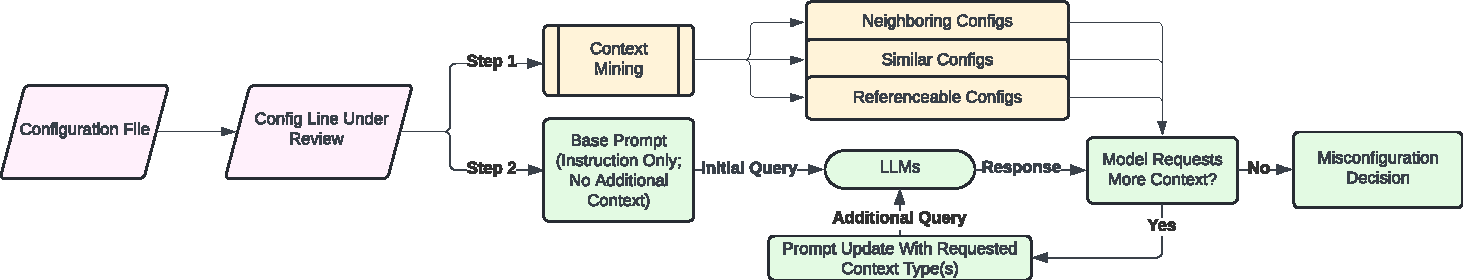
\includegraphics[width=\linewidth]{figs/cap.pdf}
    \caption{\sysname{} system overview.}
    \label{fig:overview}
\end{figure*}

We introduce a tool that tackles the aforementioned challenges via a \emph{context-aware prompting mechanism} (\sysname{}). This approach strategically manages and incorporates only the relevant parts of configurations for each line under review, ensuring that LLMs obtain the required context without succumbing to overload. 
At the same time, this line-by-line methodology provides maximum granularity and emulates the workflow of a human expert, who typically focuses on a single statement to trace its specific dependencies and impacts.
\sysname{} has two components, as
shown in Figure~\ref{fig:overview}:


% \mypara{1. Context Mining:} In this component, \sysname{} mines
% relevant context for a given configuration line under examination. 
% Our definition of relevance extends beyond configurations that are syntactically linked or physically adjacent. \aaron{``Syntactically linked'' seems synonymous with ``referenced policies and objects'' and ``physically adjacent'' seems synonymous with ``neighboring,'' so its odd to say that ``our definition [...] extends beyond [...] syntactically linked or physically adjacent.''} It also includes lines that are \textit{semantically crucial} for a correct interpretation, such as neighboring configurations, similar lines applied in different contexts, or referenced policies and objects that define key parameters.

\mypara{1. Context Mining:} In this component, \sysname{} mines relevant context for a given configuration line under examination. Our definition of relevance is comprehensive, encompassing not only the most direct forms of context—such as physically adjacent (neighboring) lines and syntactically linked (referenceable) policies—but also a more nuanced, \textit{semantically crucial} context: functionally similar lines applied in different parts of the network.

\mypara{2. Guided Prompting:} Once the relevant context has been
mined, the online component engages the LLM through an interactive prompting
process. Instead of overwhelming the model with all the extracted context at
once, \sysname{} interacts with the LLM in a guided manner.

%We now explain the challenges encountered in designing these two components and present the solutions.
We discuss these two components in detail in Sections~\ref{mining_method} and \ref{prompting_method}, respectively.